\documentclass[a4paper]{scrartcl}
\usepackage[
    fach=Informatik,
    lerngruppe={GK EF},
    typ=kl,
    klausurtyp=klausur,
    nummer=2,
    farbig,
    datumAnzeigen,
    seitenzahlen=autoGesamt,
    loesungen=seite,
    erwartungshorizontAnzeigen,
]{schule}

% Dieses Dokument ist in der Zusammenarbeit von verschiedenen
% Informatikreferendaren und Informatiklehrern entstanden.
% Der Herausgeber dieses Dokuments ist die Fachgruppe Informatische
% Bildung in NRW der Gesellschaft für Informatik.
%
% Das Dokument steht unter der Lizenz: Creative Commons by-nc-sa Version 4.0
% http://creativecommons.org/licenses/by-nc-sa/4.0/deed.de
%
% Nach dieser Lizenz darf das Dokument beliebig kopiert und bearbeitet werden,
% sofern das Folgeprodukt wiederum unter gleichen Lizenzbedingungen vertrieben
% und auf die ursprünglichen Urheber verwiesen wird.
% Eine kommerzielle Nutzung ist ausdrücklich ausgeschlossen.
%
% Die Namensnennung durch einen Verweis und die Lizenzangabe der ursprünglichen
% Urheber auf den Materialien für Schülerinnen und Schüler ist erforderlich.
%
% Die Sammlung der Dokumente steht unter
% http://ddi.uni-wuppertal.de/material/materialsammlung/
% zur Verfügung.
%
% Das LaTeX-Paket zum Setzen der Dokumente der Sammlung steht
% unter  http://www.ctan.org/pkg/schule
% zur Verfügung.

\author{Fachgruppe Informatische Bildung in NRW der Gesellschaft für Informatik}

\title{Objektorientierte Modellierung}

\date{15.05.2015}

% \usepackage[bottom=4cm]{geometry}

\begin{document}

\section*{Modellierung mit Objekten}

\begin{aufgabe}
    Der 30-jährige Dieter und seine zwei Jahre jüngere Frau Margret befinden sich im Urlaub und möchten sich jeweils einen Roller mieten. Sie sind an Manni und seinen Kollegen Franz geraten. Dieter bittet Manni, die Formalitäten zu erledigen. Manni überreicht den beiden Urlaubern jeweils ein blaues Formular, das beide in Empfang nehmen und ausfüllen. Nach dem Ausfüllen geben sie die Formulare an Franz, da Manni mittlerweile sein Lieblingslied \enquote{[Hoch auf dem gelben Wagen]} singt.

    \begin{teilaufgaben}
        \teilaufgabe Lesen Sie die obige Situationsbeschreibung.
        \teilaufgabe[10] Ermitteln Sie mit Hilfe des \emph{Verfahrens von Abbott} alle in der obigen Situationsbeschreibung vorkommenden Objekte mitsamt ihren Attributen und Methoden.
        \teilaufgabe[10] Entwerfen Sie für jedes Objekt eine Objektkarte für die Situation, unmittelbar nachdem Manni den beiden Urlaubern jeweils ein Formular übergeben hat.
        \teilaufgabe[5] Stellen Sie die Beziehungen der Objekte untereinander als Objektdiagramm dar.
    \end{teilaufgaben}
    \begin{loesung}
        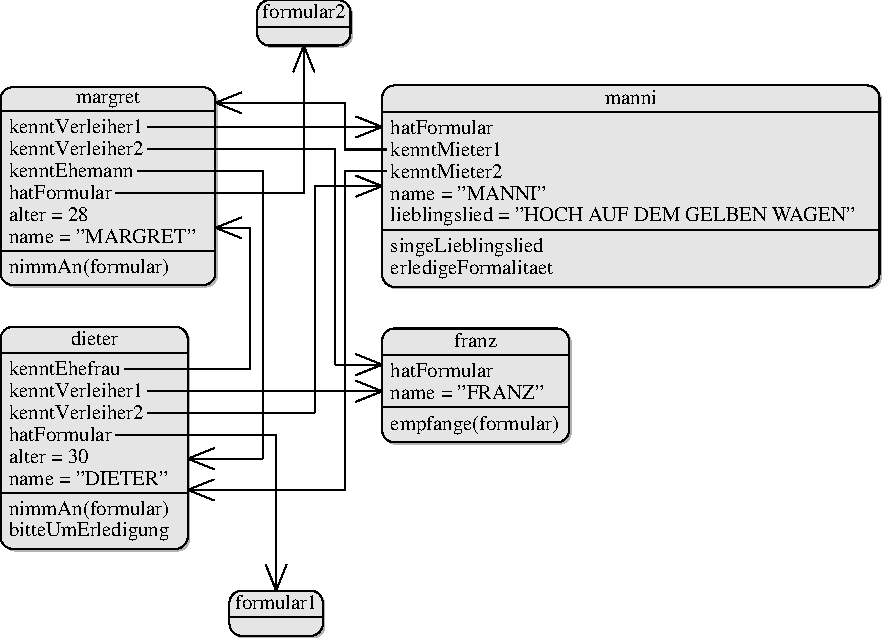
\includegraphics[scale=0.8]{aufgabe-1}
    \end{loesung}
    \begin{erwartungen}
        \erwartung{ermittelt die Objekte \texttt{margret}, \texttt{dieter}, \texttt{franz}, \texttt{manni}, \texttt{formular1} und \texttt{formular2}.}{3}
        \erwartung{ermittelt die Attribute \texttt{alter}, \texttt{hatFormular}, \texttt{lieblingslied} und ordnet sie korrekt zu.}{3}
        \erwartung{ermittelt die Methoden \texttt{nimmAn(formular)}, \texttt{erledigeFormalitaet} und \texttt{singeLied}.}{4}
        \erwartung{entwirft ein, der Situation entsprechendes, Objektdiagramm.}{5}
        \erwartung{stellt das Objektdiagramm den Konventionen entsprechend dar:
            \begin{smallitemize}
                \item Objektnamen klein
                \item Attributwerte groß
                \item Aufträge im Imperativ
                \item Präfixe bei den Attributen
                \item Anführungszeichen bei Zeichenketten
            \end{smallitemize}
            }{5}
        \erwartung{stellt die Beziehungen zwischen den Objekten vollständig und korrekt dar.}{5}
    \end{erwartungen}
\end{aufgabe}

\section*{Sequenz- und Klassendiagramme}

\begin{aufgabe}
    \scalebox{0.8}{
        \begin{sequencediagram}
            \newthread{au}{aussen}
            \newinst[]{imke}{imke}
            \newinst[]{jean}{jean}
            \newinst[2.5]{fritz}{fritz}
            \newinst[2]{wespa}{wespa24FX4}
            \newinst[]{april}{aprilF241}
            \begin{call}{au}{gibRollerZurueck}{jean}{}
                \begin{call}{jean}{empfange(hatRoller)}{fritz}{}
                \begin{call}{fritz}{gibFuellstandTank}{wespa}{0.25}
                \end{call}
                \begin{call}{fritz}{starte}{wespa}{}
                \end{call}
                \begin{call}{fritz}{gibGas}{wespa}{}
                \end{call}
                \begin{call}{fritz}{schalteAus}{wespa}{}
                \end{call}
                \end{call}
            \end{call}
        \end{sequencediagram}
    }
    \begin{teilaufgaben}
        \teilaufgabe[5] Erweitern Sie das Sequenzdiagramm um die folgende Situationsbeschreibung, die sich im Anschluss abspielen soll:
            \begin{quotation}
                Imke begutachtet ihren geliehenen Roller \enquote{AprilF241}. Sein Zustand ist offenbar, dass er kaputt ist. Sie fragt den Verleiher Fritz nach den Kosten für einen neuen Roller, der ihr \enquote{300\,\euro} antwortet.
            \end{quotation}
        \teilaufgabe[10] Modellieren Sie auf der Basis der Information, die Sie dem Sequenzdiagramm (inkl. Ihrer Erweiterung aus Aufgabenteil a) entnehmen können, ein entsprechendes Klassendiagramm mit Beziehungen und Kardinalitäten. Konstruktoren bzw. Destuktoren müssen nicht mit angegeben werden. Ergänzen Sie die Klassen aber um geeignete Attribute.
    \end{teilaufgaben}
    \begin{loesung}
        \begin{teilaufgaben}
            \teilaufgabe Erweitertes Sequenzdiagramm:

                \scalebox{0.6}{
                    \begin{sequencediagram}
                        \newthread{au}{außen}
                        \newinst[2]{imke}{imke}
                        \newinst[]{jean}{jean}
                        \newinst[2.5]{fritz}{fritz}
                        \newinst[2]{wespa}{wespa24FX4}
                        \newinst[]{april}{aprilF241}
                        \begin{call}{au}{gibRollerZurueck}{jean}{}
                            \begin{call}{jean}{empfange(hatRoller)}{fritz}{}
                                \begin{call}{fritz}{gibFuellstandTank}{wespa}{0.25}
                                \end{call}
                                \begin{call}{fritz}{starte}{wespa}{}
                                \end{call}
                                \begin{call}{fritz}{gibGas}{wespa}{}
                                \end{call}
                                \begin{call}{fritz}{schalteAus}{wespa}{}
                                \end{call}
                            \end{call}
                        \end{call}
                        \begin{call}{au}{begutachteRoller}{imke}{}
                            \begin{call}{imke}{zustand}{april}{\diastring{kaputt}}
                            \end{call}
                            \begin{call}{imke}{kostenNeu}{fritz}{\diastring{300 Euro}}
                            \end{call}
                        \end{call}
                    \end{sequencediagram}
                }
            \teilaufgabe Klassendiagramm:

                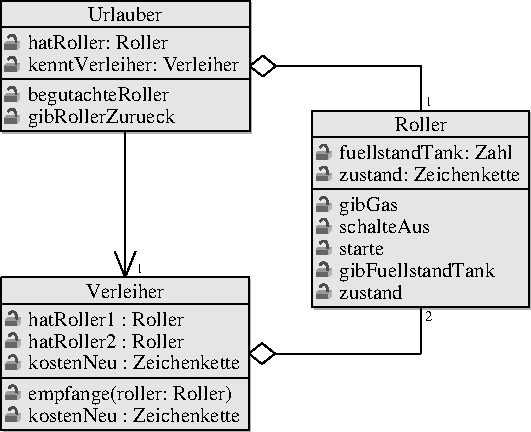
\includegraphics[scale=0.8]{aufgabe-2}
        \end{teilaufgaben}
    \end{loesung}
    \begin{erwartungen}
        \erwartung{gibt die Aufträge \texttt{begutachteRoller}, \texttt{zustand} und \texttt{kostenNeu}, sowie die zugehörigen Antworten an und erweitert das Diagramm entsprechend.}{5}
        \erwartung{modelliert ein zu den vorherigen Aufgaben konsistentes Klassendiagramm.}{8}
        \erwartung{stellt das Klassendiagramm unter Berücksichtigung der geltenden Vereinbarungen korrekt dar.}{2}
    \end{erwartungen}
\end{aufgabe}

\begin{aufgabe}
    Implementieren Sie die Methode \texttt{empfange(roller)}. Der Methodenkopf ist vorgegeben, Sie müssen Anfragen/Aufträge einfügen.
    \begin{lstlisting}[language=python,gobble=8],
        # Methode empfange
        def empfange (self, roller):

    \end{lstlisting}
    \begin{loesung}
        \begin{lstlisting}[language=python,gobble=12],
            # Methode empfange
            def empfange (self, roller):
                self.hatRoller= roller
                print(roller.gibFuellstandTank())
                roller.starte()
                roller.gibGas()
                roller.schalteAus()
        \end{lstlisting}
    \end{loesung}
    \begin{erwartungen}
        \erwartung{implementiert eine dem Klassendiagramm entsprechende Methode unter Verwendung der notwendigen Anfragen und Aufträge.}{8}
        \erwartung{wendet beim Implementieren die korrekte Syntax an.}{2}
    \end{erwartungen}
\end{aufgabe}

\end{document}